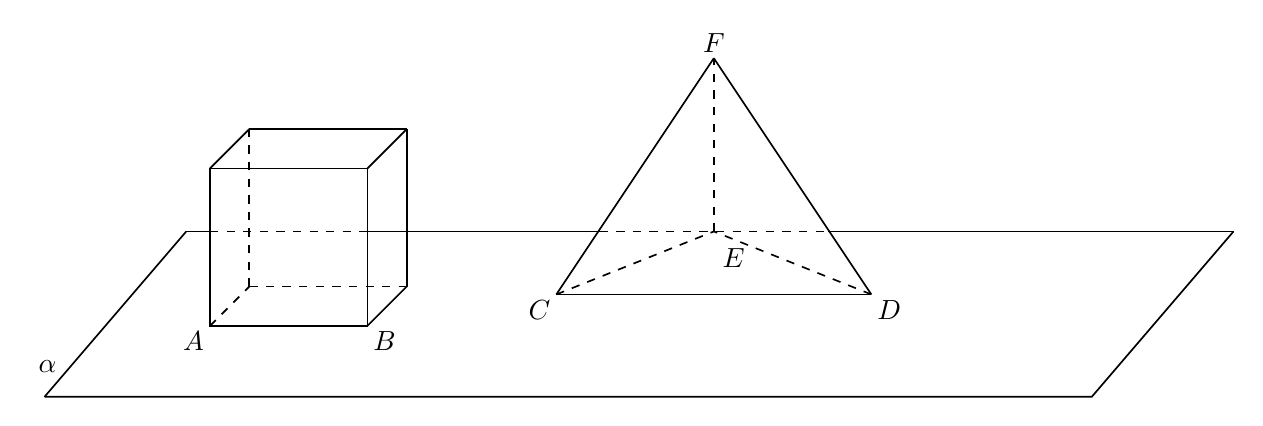
\begin{tikzpicture}[x=1cm,y=1cm,font=\normalsize,
  edge/.style={draw=black,solid,line width=.6pt},
  hide/.style={draw=black,dashed,line width=.6pt}]
% Ground plane alpha: front edge solid, back edge at E height
\coordinate (P1) at (-4.3,-1.5);
\coordinate (P2) at (9.0,-1.5);
\coordinate (P3) at (10.8000000000,0.6000000000);
\coordinate (P4) at (-2.5000000000,0.6000000000);
\draw[edge] (P1)--(P2)--(P3);
\draw[edge] (P4)--(P1);
% back edge: solid outside solids, dashed where hidden
\draw[edge] (P4)--(-2.2,0.6);
\draw[hide] (-2.2,0.6)--(-0.2,0.6);
\draw[edge] (-0.2,0.6)--(2.75,0.6);
\draw[hide] (2.75,0.6)--(5.65,0.6);
\draw[edge] (5.65,0.6)--(P3);
% cube: front face A,B, top face
\coordinate (A) at (-2.2,-0.6);
\coordinate (B) at (-0.2,-0.6);
\coordinate (A2) at (-2.2,1.4);
\coordinate (B2) at (-0.2,1.4);
\coordinate (A3) at (-1.7,1.9);
\coordinate (B3) at (0.3,1.9);
\draw[edge] (A)--(B)--(B2)--(A2)--cycle;
\draw[edge] (A2)--(A3);
\draw[edge] (B2)--(B3);
\draw[edge] (A3)--(B3);
\draw[hide] (A)--(-1.7,-0.1);
\draw[edge] (B)--(0.3000000000,-0.1000000000);
\draw[edge] (0.3000000000,-0.1000000000)--(B3);
\draw[hide] (-1.7,-0.1)--(0.3,-0.1);
\draw[hide] (-1.7,-0.1)--(-1.7,1.9);
% tetrahedron CDE base on plane, F apex
\coordinate (C) at (2.2,-0.2);
\coordinate (Dd) at (6.2,-0.2);
\coordinate (E) at (4.2,0.6);
\coordinate (F) at (4.2,2.8);
\draw[edge] (C)--(Dd);
\draw[edge] (C)--(F);
\draw[edge] (Dd)--(F);
\draw[hide] (C)--(E);
\draw[hide] (Dd)--(E);
\draw[hide] (E)--(F);
\node[below left,inner sep=2pt] at (A) {$A$};
\node[below right,inner sep=2pt] at (B) {$B$};
\node[below left,inner sep=2pt] at (C) {$C$};
\node[below right,inner sep=2pt] at (Dd) {$D$};
\node[below right,inner sep=2pt,xshift=1pt,yshift=-4pt] at (E) {$E$};
\node[above,inner sep=2pt] at (F) {$F$};
\node[below left,inner sep=4pt,xshift=0pt,yshift=6pt] at (-4.0,-1.1) {$\alpha$};
\end{tikzpicture}
